% !TeX spellcheck = nl_NL
\chapter{\IfLanguageName{dutch}{Stand van zaken}{State of the art}}
\label{ch:stand-van-zaken}

% Tip: Begin elk hoofdstuk met een paragraaf inleiding die beschrijft hoe
% dit hoofdstuk past binnen het geheel van de bachelorproef. Geef in het
% bijzonder aan wat de link is met het vorige en volgende hoofdstuk.

% Pas na deze inleidende paragraaf komt de eerste sectiehoofding.

Dit hoofdstuk gaat dieper in op de relevante inhoud van de GDPR voor dit onderzoek, en de mogelijke praktische oplossingen. 
Het einddoel is niet om een samenvatting te geven over de theoretische kant van de regelgeving, maar praktische oplossingen te bieden hoe bedrijven zich beter te kunnen aanpassen aan de GDPR. 
Het is echter noodzakelijk enkele facetten toe te lichten zodat de lezer de nodige theoretische kennis heeft.
Dit hoofdstuk dient als theoretische achtergrond om in hoofdstuk 3 GDPR-maatregelen voor te stellen en in hoofdstuk 4 die in de praktijk om te zetten.
 
 
\section{{GDPR Theoretisch}}

De EU General Data Protection Regulation (GDPR) is een regelgeving ontworpen door de EU, met als bedoeling een eerste stap te bieden naar het teruggeven van controle aan de EU-burgers, over wat er met hun persoonlijke gegevens gebeurt Eucom2018 . 

\subsection{Juridisch}
De Europese commissie beschrijft de juridische aspecten van gegevensbescherming in \autocite{Lusignan2014} als volgt.

\begin{itemize}
    \item \textbf{Grondrecht}: Het Handvest van de grondrechten van de EU bepaalt dat EU-burgers recht hebben op bescherming van hun persoonsgegevens.
    \item \textbf{Wetgeving}: 
    \subitem \textbf{De algemene verordening gegevensbescherming} (GDPR): 
    Verordening (EU) 2016/679 betreffende de bescherming van natuurlijke personen in verband met de verwerking van persoonsgegevens en betreffende het vrije verkeer van die gegevens.
    \subitem \textbf{De politierichtlijn}: 
    Richtlijn (EU) 2016/680 betreffende de bescherming van natuurlijke personen in verband met de verwerking van persoonsgegevens door bevoegde autoriteiten met het oog op de voorkoming, het onderzoek, de opsporing en de vervolging van strafbare feiten of de tenuitvoerlegging van straffen, en betreffende het vrije verkeer van die gegevens.
   
\end{itemize}

Verder hebben de EU-landen nationale autoriteiten voor gegevensbescherming aangewezen die dienen toezicht te houden op de bescherming van persoonsgegevens. Voor België is dit: 

\quad \textit{Gegevensbeschermingsautoriteit / Commission de la protection de la vie privée. \\ \quad Rue de la Presse 35 1000 Brussel \\  \quad Website: http://www.privacycommission.be/ \\ 
    \quad Art 29 WP Vice-President: Willem DEBEUCKELAERE, President of the Belgian Privacycommission} 

\begin{figure}[h]
	\centering
	\begin{subfigure}{0.4\textwidth}
		\centering
		
\includegraphics[width=.4\linewidth]{gba.png}
		\caption{Gegevensbeschermingsautoriteit.}
	\end{subfigure}
	\begin{subfigure}{0.5\textwidth}
		\centering
		
\includegraphics[width=.4\linewidth]{CPVP.jpg}
		\caption{Commission de la vie privée}
	\end{subfigure}%
	\caption{Autoriteit voor gegevensbescherming in België. (Vlaanderen en Wallonië)}
\end{figure}

Tot slot is er nog een Europees Comité voor gegevensbescherming. In bron eucom wordt gesteld dat het comité ruime bevoegdheden heeft om geschillen tussen de nationale toezichthoudende autoriteiten te beslechten, adviezen te geven en richtsnoeren vast te stellen over essentiële aspecten van de algemene verordening gegevensbescherming en de politierichtlijn.

%europa.eu/european-union/about-eu/institutions-bodies/european-data-protection-supervisor_nl)


Hierbinnen is een Europees toezichthouder aangesteld voor de gegevensbescherming. Zijn rol is om erop toe te zien dat de EU-instellingen en -organen de privacy van de burgers respecteren bij de verwerking van persoonsgegevens. Tijdens het opstellen van dit onderzoek (2019) is dit \textit{Giovanni Buttarelli}. 
\\ Hij controleert dus niet zozeer zelfstandige organisaties, maar de instellingen die gegevens verwerken. 


\subsection{Voor wie? }
Niet elke organisatie moet rekening houden met de GDPR. Er zijn binnen de regelgeving enkele voorwaarden opgesteld. Bijvoorbeeld: als gegevens van gebruikers noch verwerkt worden, noch worden bijhouden, komt de organisatie er niet mee in contact. 

Er zijn bepaalde voorwaarden geformuleerd: 
\subsubsection{Materieel toepassingsgebied.}
Artikel 2 van de GDPR spreekt over het materieel toepassingsgebied. Aangezien het artikel in rechtstaal geschreven is, brengt een definitie van de GBA (gegevensbeschermingsautoriteit) meer duidelijkheid. 

\textit{Deze verordening is van toepassing op de geheel of gedeeltelijk geautomatiseerde verwerking, alsmede op de niet-geautomatiseerde verwerking van persoonsgegevens die in een bestand zijn opgenomen of die bestemd zijn om daarin te worden opgenomen.}

\subsubsection{Territoriaal toepassingsgebied}
In de eerste plaats is de GDPR een Europese regelgeving. Dit betekent echter niet dat er bij niet-Europese organisaties geen rekening mee moet gehouden worden. Er zijn twee gevallen te onderscheiden: 

\begin{itemize}
	\item De verwerkingsverantwoordelijke is gevestigd in de EU. 
	\subitem In dit geval is de GDPR van toepassing, en moet bij het bijhouden en verwerken van gegevens aan de regelgeving voldaan worden. 
	\item De verwerkingsverantwoordelijke is gevestigd buiten de EU. 
	\subitem In dit geval moet gekeken worden naar de gebruikers van wie gegevens verwerkt worden. Als de gegevens bijgehouden of verwerkt worden van ingezetenen van de EU blijft de regelgeving van kracht. 
\end{itemize}

\subsection{{Begrippen: GDPR}} 
Verder in dit onderzoek zullen specifieke termen die binnen de GDPR beschreven staan gebruikt worden.
In artikel 4 van de GDPR staan de juridische definities van die termen. Hier volgt wat extra toelichting bij de belangrijkste (\textcite{Parlement2016}). 

\subsubsection{Persoonsgegevens} 
Definitie: alle informatie over een geïdentificeerde of identificeerbare natuurlijke persoon ("\textbf{de betrokkene}"); als identificeerbaar wordt beschouwd een natuurlijke persoon die direct of indirect kan worden geïdentificeerd, met name aan de hand van een identificator zoals een naam, een identificatienummer, locatiegegevens, een online identificator of van een of meer elementen die kenmerkend zijn voor de fysieke, fysiologische, genetische, psychische, economische, culturele of sociale identiteit van die natuurlijke persoon.

 Als verder in dit onderzoek wordt gesproken over persoonlijke data, persoonsgegevens, persoonlijke gegevens, gaat het over data die bovenstaande definitie volgt.
 
  Merk op:
  \\ Ook gegevens die indirect een persoon kunnen identificeren worden als persoonlijke info beschouwd. 
 
 Voorbeeld: school, hobby, leeftijd.
 \\ Deze drie gegevens zijn op zichzelf, alleenstaand, niet genoeg om een persoon te identificeren.
 Maar als we de drie nu combineren, kan het in bepaalde gevallen leiden tot identificatie van een persoon. Stel, hij/zij gaat naar een kleine dorpsschool, is 9 jaar en beoefent judo. In veel gevallen zal dit te herleiden zijn tot één persoon, en worden dit indirect persoonlijke gegevens. 

Er zal vaak ter sprake komen dat de persoonsgegevens \underline{\textit{verwerkt}} worden, de definitie hiervan luidt als volgt: een bewerking of een geheel van bewerkingen met betrekking tot persoonsgegevens of een geheel van persoonsgegevens, al dan niet uitgevoerd via geautomatiseerde procedés, zoals het verzamelen, vastleggen, ordenen, structureren, opslaan, bijwerken of wijzigen, opvragen, raadplegen, gebruiken, verstrekken door middel van doorzending, verspreiden of op andere wijze ter beschikking stellen, aligneren of combineren, afschermen, wissen of vernietigen van gegevens.

In het vervolg van dit onderzoek zal regelmatig verwezen worden naar persoonlijke gegevens als \textbf{PII}. Dit is de afkorting voor Personally Identifiable Information.

\subsubsection{Anonimiseren}
Het verwerken van gegevens op zodanige wijze dat alle persoonsgegevens verwijderd/onleesbaar gemaakt zijn. 

\subsubsection{Pseudonimisering} 
Het verwerken van persoonsgegevens op zodanige wijze dat de persoonsgegevens niet meer aan een specifieke betrokkene kunnen worden gekoppeld zonder dat er aanvullende gegevens worden gebruikt. Mits deze aanvullende gegevens apart worden bewaard en technische en organisatorische maatregelen worden genomen om ervoor te zorgen dat de persoonsgegevens niet aan een geïdentificeerde of identificeerbare natuurlijke persoon worden gekoppeld. 

\subsubsection{Toestemming} 
De regelgeving is er in de eerste plaats gekomen om mensen te beschermen. Al te vaak werd in het verleden op een dubieuze manier toestemming gevraagd voor de verwerking van persoonsgegevens, en verstonden de betrokken gebruikers niet wat dat allemaal inhield. Daarom stelt de EU nu dat gebruikers heel duidelijk moeten weten welke data ze vrijgeven en wat er met die data mag/zal gedaan worden, en dit moet gepresenteerd worden in ondubbelzinnige, begrijpbare taal.
Daarnaast moet toestemming specifiek zijn.
\\ Als voorbeeld: een hokje om aan te vinken: “Hierbij stem ik in om al mijn persoonlijke info ter beschikking te stellen aan de organisatie”, is geen enkel geval specifiek genoeg en verboden.\\ Definitie \textit{toestemming van de betrokkene}: elke vrije, specifieke, geïnformeerde en ondubbelzinnige wilsuiting waarmee de betrokkene door middel van een verklaring of een ondubbelzinnige actieve handeling hem betreffende verwerking van persoonsgegevens aanvaardt. 

\subsubsection{Data protection by design}
Deze Engelse term wordt vrij vertaald als databescherming bij opzet. Deze benadering impliceert dat privacy en gegevens-beveiling uitgevoerd wordt vanaf het eerste moment dat gegevens verwerkt/bijhouden worden, en dit blijft uitgevoerd worden doorheen de volledige levenscyclus van die gegevens. 

\subsubsection{Inbreuken} 
Het moet ten alle koste vermeden worden, maar het is niet uitgesloten dat bepaalde persoonsgegevens ongewild worden verspreid. Denk aan hackers, data-leaks, enzoverder.
\\ De definitie wordt als volgt gesteld: een inbreuk op de beveiliging die per ongeluk of op onrechtmatige wijze leidt tot de vernietiging, het verlies, de wijziging of de ongeoorloofde verstrekking van of de ongeoorloofde toegang tot doorgezonden, opgeslagen of anderszins verwerkte gegevens. 

\subsection{Rollen}
Binnen de GDPR zijn verschillende partijen te onderscheiden. Neem als voorbeeld een KMO die gegevens van gebruikers verzamelt. Dan valt een onderscheid te maken in rol tussen de persoon van wie de gegevens verwerkt worden, en de verantwoordelijke binnen de organisatie die de gegevens verwerkt. Maar als er binnen de kmo ook gegevens worden bijgehouden van personeelsleden valt dit ook onder de regelgeving. Dat zijn dus al drie totaal verschillende rollen van waaruit in contact kan gekomen worden met de GDPR. 

De belangrijkste rollen worden hieronder beschreven. 

\subsubsection{Betrokkene}
De definitie van de betrokkene staat beschreven onder 2.1.3 Begrippen; persoonsgegevens. Dit stelt de gebruiker voor van wie een organisatie de gegevens wil bijhouden of verwerken. 

\subsubsection{Verwerkingsverantwoordelijke}
De voornaamste rol van de verwerkingsverantwoordelijke is het bepalen van de doelen en motivatie voor het verwerken van de persoonlijke gegevens. Dit kunnen in realiteit meerdere mensen zijn. Belangrijk is dat deze persoon verantwoordelijk wordt geacht acties te ondernemen om het verzamelen en verwerken van data GDPR-compliant te maken. 
Dit kan bijvoorbeeld door het aanstellen van een DPO (zie verder), en is in praktijk vaak de zaakvoerder.  

\subsubsection{DPO}
Data Protection Officer. Een verantwoordelijke aangesteld om de strategie te bepalen hoe data op een goede en veilige manier kan verzameld worden. Hij houdt ook toezicht op de implementatie van deze strategie.
Enkel onder bepaalde voorwaarden is het aanstellen van een DPO verplicht, maar ook als het niet verplicht is, is het ten zeerste aan te raden zodat de verantwoordelijkheid duidelijk bij een bepaald persoon ligt. 

\underline{Voorwaarden verplicht aanstellen DPO} :  \\
Voor overheidsbedrijven en bedrijven die strafrechtelijke data verwerken geld de verplichting sowieso. Behoort de onderneming niet tot één van die twee is het verplicht indien: 'een verwerkingsverantwoordelijke of de verwerker hoofdzakelijk is belast met verwerkingen die vanwege hun aard, hun omvang en/of hun doeleinden regelmatige en stelselmatige observatie op grote schaal van betrokkenen vereisen'. \textcite{ConXioN2017} \\
Dit is echter geen sluitende definitie en voor interpretatie vatbaar. Daarom heeft de werkgroep rond de wetgeving extra toelichting gegeven, waarin voorbeelden worden opgesomd. 

Een voorbeeld van de werkgroep van dataverwerking op schaal: verwerken van patiëntendata door ziekenhuizen.  

   \begin{figure}[h]
	\centering
	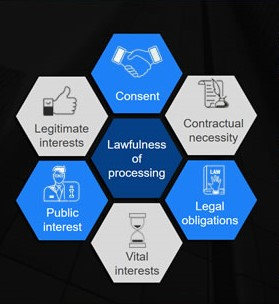
\includegraphics[scale=0.7]{six_pilars_processing.jpg}
	\caption{6 voorwaarden om rechtmatig gegevens te verwerken, schematische voorstelling. \textcite{IScoop2017}}
\end{figure}

\subsection{Rechtmatigheid van verwerking}
Als organisatie of rechtspersoon in het algemeen moet er van uitgegaan worden dat het verzamelen van persoonsgegevens standaard verboden is. Als er toch gebruik van wil gemaakt worden, moet aan minstens één van de volgende voorwaarden voldaan worden. \textcite{Commissie2016}
\begin{itemize}
    \item \textbf{Toestemming:} Gegevensverwerking kan enkel indien er de betrokkene expliciet toestemming (zie sectie 2.1.2) heeft gegeven om (beperkt) met zijn persoonlijke data aan de slag te gaan en die te verwerken. \\
    
    \item \textbf{Noodzaak}: De verwerking is noodzakelijk voor de uitvoering van een overeenkomst waarbij de betrokkene partij is, of om op verzoek van de betrokkene vóór de sluiting van de overeenkomst maatregelen te nemen. \\
    
    \item \textbf{Voldoen aan wettelijke verplichting }: de verwerking is noodzakelijk om te voldoen aan een wettelijke verplichting die op de verwerkingsverantwoordelijke rust; \\
    
     \item \textbf{Bescherming van vitale belangen}:  de verwerking is noodzakelijk om de vitale belangen van de betrokkene of van een andere natuurlijke persoon te beschermen. \\
    
    \item \textbf{Algemeen belang}: de verwerking is noodzakelijk voor de vervulling van een taak van algemeen belang of van een taak in het kader van de uitoefening van het openbaar gezag dat aan de verwerkingsverantwoordelijke is opgedragen. \\
    
     \item \textbf{Behartiging van de belangen}: de verwerking is noodzakelijk voor de behartiging van de gerechtvaardigde belangen van de verwerkingsverantwoordelijke of van een derde, behalve wanneer de belangen of de grondrechten en de fundamentele vrijheden van de betrokkene die tot bescherming van persoonsgegevens nopen, zwaarder wegen dan die belangen, met name wanneer de betrokkene een kind is. \\
\end{itemize}



\subsection{Rechten en toestemming van de betrokkene}
In sectie 2.1.3 wordt toegelicht wat het volgens de GDPR begrepen wordt onder toestemming van de gebruiker. Hier volgt extra informatie rond dit onderwerp. 

 Toestemming is één van de zes voorwaarden (zie 2.1.5) waar aan moet worden voldaan om te kunnen overgaan tot rechtmatige gegevensverwerking. De GDPR focust vooral op de begrijpelijkheid en duidelijkheid wanneer en waarvoor de gebruiker toestemming geeft. 
Er zijn enkele voorwaarden opgenomen in de wetgeving waar de toestemming van de betrokkene moet aan voldoen. 
\begin{itemize}
	\item  Als  gegevens verwerkt worden op basis van toestemming, moet een organisatie ten alle tijde bewijs kunnen leveren dat de betrokkene specifiek voor elke soort gegevens toestemming heeft gegeven. 
	\item  Het verzoek dient in een \textbf{begrijpelijke en gemakkelijk toegankelijke vorm en in duidelijke en eenvoudige taal} opgesteld te zijn. 
	\item  
	De toestemming kan ten alle tijde \textbf{ingetrokken worden}, en dit proces is even eenvoudig als het het geven ervan. 
\end{itemize}

Nadat de betrokkene toestemming heeft gegeven tot het verwerken van zijn gegevens, behoudt hij/zij bepaalde rechten. Hieronder worden kort enkele van deze rechten verder toegelicht die van belang zijn voor dit onderzoek. 

\subsubsection{Recht van inzage}
Indien een verwerkingsverantwoordelijke de persoonsgegevens van een betrokkene verwerkt, heeft deze laatste volgens artikel 15 van de GDPR het recht deze gegevens in te
zien en hieromtrent extra informatie op te vragen.
De verwerkingsverantwoordelijke dient hier kosteloos gevolg aan te geven, tenzij de
verzoeken van de betrokkene ongegrond of buitensporig zijn. Bij repetitieve herhaling
mag de verwerkingsverantwoordelijke hiervoor een administratieve vergoeding vragen of
weigeren gevolg te geven aan het verzoek. (\textcite{Commissie2016})

\subsubsection{Recht tot verwijdering}

Naast een aanvraag om inzage te krijgen in de bijgehouden persoonsgegevens van zichzelf, kan gevraagd worden om alle bijgehouden gegevens die terug te leiden zijn naar deze persoon, te verwijderen. Opnieuw moet de verwerkingsverantwoordelijke hier kosteloos gevolg aan geven. (\textcite{Commissie2016}) 

\section{Technische Achtergrondinformatie}
Voor de volgende hoofdstukken is een bepaalde technische voorkennis vereist. Hieronder volgt een introductie met uitleg over de gebruikte termen en onderdelen. 

\subsection{Technische begrippen}
\subsubsection{API}
Een API of Application Program Interface is een set van routines, protocollen en tools om software appplicaties te maken. Een api specifiëert hoe de interactie tussen twee software componenten gebeurt. 
\textcite{QuinStreet2019}

\subsubsection{SDK}
Een SDK of een Software Development Kit is een 'programmeer-pakket' dat een programmeur ertoe in staat stelt om applicaties te ontwikkelen voor een bepaald platform. \textcite{QuinStreet2019}

\subsubsection{JSON}
JSON of JavaScript Object Notation, in een formaat om elektronisch data uit te wisselen, gebaseerd op de programeertaal JavaScript. \textcite{QuinStreet2019}

\subsubsection{Machine Learning}
In de context van computerwetenschappen wordt met machine learning een type van data-analyse bedoeld, 
dat algoritmes gebruikt om uit die data bij te leren en bijgevolg betere analyses te maken. \textcite{QuinStreet2019}, dit is een onderdeel van het algemenere woord Artificiële intelligentie. 

\subsection{Digitale opslag gegevens}
In de GDPR wordt gesproken over persoonsgegevens en persoonlijke data. Data die moet beschermd worden. Maar binnen de bedrijfs- en infomaticawereld kan er niet van uitgegaan worden dat data is opgedeeld in persoonlijke en niet-persoonlijke data. Eén van de uitdagingen binnnen de GDPR is net dit onderscheid te maken binnen opgeslagen gegevens. \\

\subsubsection{Databases} 
Gegevens kunnen op allerlei manieren verzameld en verwerkt worden, en een manier om ze uiteindelijk op te slaan is in een database. Een database is een digitale verzameling van ruwe data in tabellen. Een database moet het mogelijk maken een grote hoeveelheid gegevens gemakkelijk en snel te benaderen. 

\subsubsection{Structurele vs. niet-structurele data.}
Binnen databases kan data in verschillende vormen voorkomen. Er wordt voor dit onderzoek een onderscheid gemaakt tussen structurele en niet structurele data. 

Structurele data is data die altijd in een bepaalde vorm, of structuur wordt aangeboden. Denk aan een telefoonnummer of een emailadres. 

Niet-structurele data heeft geen vaste vooropgesteld vorm of structuur. Dit komt vaak voor in de vorm van langere stukken tekst.\\

Een voorbeeld ter verduidelijking: \\
Op een bepaalde webapplicatie wordt gevraagd naar registratiegegevens. Er zijn drie velden die moeten ingevuld worden:\\ 'Naam', 'emailadres', en 'extra opmerkingen'. \\
Er wordt respectievelijk ingevuld: \\'John Smith', 'j.s@demo.com' en 'Gelieve me geen emails te sturen met reclame, ik vind dat niet leuk. O ja, kunnen jullie me even opbellen, ik heb nog een vraag'. 

Naam en emailadres zijn voorbeelden van structurele data, aangezien deze een vooraf bepaalde vorm zullen volgen. 
Extra opmerkingen is een voorbeeld van niet-structurele data. De vorm van het antwoord is niet vooraf bepaald. 

\subsection{InSites Consulting}
InSites Consulting is een marktonderzoeksbureau (met ongeveer 300 werknemers verspreid over 7 landen). InSites onderzoekt op basis van opdrachten van klanten waarom bepaalde producten minder/beter scoren op de markt, hoe populair een bepaald merk is, enzoverder. Hiervoor wordt zowel kwantitatief als kwalitatief onderzoek uitgevoerd in de vorm van openbare discussies en vragenlijsten. Dit onderzoek wordt uitgevoerd op een brede groep van participanten, wereldwijd. Bijgevolg komt InSites in \textbf{grote mate in contact met persoonlijke informatie}. \\
Bijvoorbeeld: een marktonderzoek naar shampoo, waar participanten elke dag een foto posten van hun haar. Hierbij kan verondersteld worden dat deze foto's gezichten zullen bevatten, wat persoonlijke informatie is. 

\subsection{InSites-Square}
Het digitale product waarop dit kwalitatief en kwantitatief onderzoek wordt uitgevoerd heet 'InSites-Square'. In het vervolg van dit hoofdstuk zal hiernaar gerefereerd worden als de 'Square'. 
De Square is een online platform, met enkele duizenden participanten, voor verschillende marktonderzoeken. 
Voor InSites Consulting is het de bedoeling om de 'Square' zo goed mogelijk te laten voldoen aan de eisen van de GDPR. Eén van de grootste uitdagingen hierbij, is het vinden van persoonlijke informatie in niet-gestructureerde data, wat het hoofdonderdeel van dit uitgewerkte hoofdstuk is, naast enkele andere implementaties die kunnen leiden tot een meer GDPR-aanvaardbaar platform.  

\chapter{\IfLanguageName{dutch}{Maatregelen}{}}
\label{ch:Maatregelen}
In vorig hoofdstuk is het theoretisch aspect van de GDPR uitgelegd, en is er enige technische achtergrondinformatie verschaft. In dit hoofdstuk wordt dieper ingegaan op welke maatregelen precies kunnen genomen worden om een onderneming te laten voldoen aan de regelgeving. Er worden \textbf{organisatorische} maatregelen besproken, maar de nadruk ligt op de \textbf{technische maatregelen}. 

Enkele van deze maatregelen, die een technische uitdaging vormen om op te lossen, zullen dieper uitgewerkt worden in hoofdstuk 4. Deze maatregelen zijn: 
\begin{itemize}
    \item 3.6 Dataretentie
    \item 3.8 Verwerken niet-structurele data
\end{itemize}

Tot slot wordt een overzicht gegeven in een tabel van alle mogelijke maatregelen. 

Opmerking: In de regelgeving wordt een verschil gemaakt tussen verschillende types organisaties. Bijvoorbeeld: of er al dan niet in grote mate persoonlijke gegevens verwerkt worden. Afhankelijk hiervan zijn de regels minder streng/strenger (zie hoofdstuk 2). In dit werk wordt gefocust op kmo's die een grote hoeveelheid persoonlijke gegevens op geautomatiseerde manier verwerken.  

\section{Privacyscan}
Een eerste maatregel die een bedrijf kan ondernemen is een een privacyscan, ook wel een Data Protection Impact Assessment (DPIA) genoemd, of in het Nederlands: Gegevensbeschermingseffectbeoordeling. 

In sommige gevallen is het uitvoeren van een privacyscan verplicht: 
Wanneer de verwerking van gegevens een 'waarschijnlijk hoog risisco' inhoudt. Dit is een grijze zone, daarom wordt in overweging 75 van de GDPR extra informatie hieromtrent gegeven. Enkele voorbeelden van wanneer er volgens de GDPR sprake is van groot risico: 

\begin{itemize}
	\item De verwerking van gegevens kan leiden tot discriminatie
	\item De gegevens bevatten beroepsgeheim
	\item Wanneer gegevens worden verwerkt met politieke opvattingen, religie, ... 
	\item Voor de volledige lijst, raadpleeg overweging 75 in de bijlage. 
\end{itemize}

De definitie van een privacyscan is volgens \textcite{ConXioN2017} een proces dat ertoe strekt om risico’s te evalueren in verband met de rechten en vrijheden van natuurlijke personen, die ontstaan of dreigen te ontstaan naar aanleiding van de verwerking van persoonsgegevens, evenals om de mogelijkheden tot beheersing van deze risico’s te evalueren.

\section{Sensibilisering personeel}
Naast alle stappen (die verder in de werk beschreven worden) om de onderneming zijn data in databases, cloud services, enzoverder te beschermen, is het ook belangrijk dat het personeel op de hoogte is van wat wel en niet mag. Er moet vermeden worden dat de software van het bedrijf tot in de puntjes beveiligd is, maar een werknemer met toegang tot persoonlijke gegevens en kopie neemt van de database op een usb-stick en die laat rondslingeren. 

Dit kan op verschillende manieren aangepakt worden.
 Door een presentatie te geven/ een online presentatie ter beschikking stellen, met alle info rond de GDPR, wat wel en niet kan, en met wat de GDPR-beleid  van het bedrijf is. 

Ook zijn op het internet allerhande bewustzijnstrainingen voorhanden. Deze trainingen hebben als doel er voor te zorgen dat de werknemer even stil staat bij de GDPR, weet wat dit voor hem/haar betekent, en er in de toekomst rekening mee zal houden.  

Door regelmatig testen uit te voeren, zoals interne phising\footnote{Met phising wordt volgens QuinStreet2019 bedoeld het uitsturen van een email/tekstbericht naar een internetgebruiker, zich valselijk voordoend als een legitieme onderneming, om de gebruiker uit te lokken ongewild persoonlijke gegevens, bankgegevens, enzoverder vrij te geven.} campagnes. Er zijn hier vele mogelijkheden om als werkgever of DPO mee aan de slag te gaan. 

\section{Contractbeheer}
Als een onderneming persoonlijke gegevens verwerkt, en deze ook deelt met andere services/bedrijven (bijvoorbeeld cloud services), is de onderneming verplicht hierover contractuele afspraken over op te stellen. Dus ook bestaande contracten met zogenaamde 'third-parties' dienen te worden aangepast aan de GDPR. 

Indien hier niet aan voldaan wordt, zal in het geval er een gegevenslek of misdrijf plaatsvindt, de onderneming die de gegevens in de eerste plaats verwerkt heeft, verantwoordelijk gesteld worden. 

Een voorbeeld: 
Autogarage 'Jan en Zoon' vraagt aan elke klant een blad met gegevens in te vullen. (Naam, emaildres, adres, enzoverder). De onderneming deelt deze informatie met een onderzoeksbureau 'De MarktVerkenners' die willen weten in welke dorpen de meeste auto's stuk gaan. Als er geen contract is tussen 'Jan en Zoon' en 'De Marktverkenners' waarin voldaan wordt aan alle eisen van de GDPR, zal in het geval van een gegevenslek bij 'De Marktverkenners', toch de autogarage 'Jan en zoon' aansprakelijk gesteld worden.

\section{Privacy Policy mededeling}
De meeste organisaties beschikken over een privacybeleid. Dit dient (binnen de strekking van de GDPR) om de gebruiker, vooraleer hij/zij persoonlijke info achterlaat, te informeren in welke mate die gegevens zullen bijgehouden worden, en hoe ze worden verwerkt. De GDPR stelt echter enkele nieuwe voorwaarden om de gebruiker te beschermen, vooral tegen het feit dat deze policies vaak onduidelijk zijn, en de gebruiker niet weet waarmee hij akkoord gaat.
Artikel 12, 13 en 14 (VERWIJZING) van de GDPR geven uitgebreide instructies hoe het privacybeleid opgesteld moet worden, en op die inhoud zal niet tot in detail worden ingegaan tijdens dit onderzoek; een goede privacy policy mededeling kan wel worden omschreven in vier eigenschappen. 

\begin{itemize}
	\item Moet geschreven zijn in beknopte, transparante, begrijpelijke en toegankelijke vorm.
	\item Moet duidelijke en ondubbelzinnige taal bevatten, die eenduidig te interpreteren is. 
	\item Moet gratis aangeboden worden.
	\item Moet tijdig aangeboden worden.
\end{itemize}

Een technische maatregel die hier wel zou kunnen genomen worden, is ervoor zorgen dat de privacy policy mededeling correct en duidelijk verschijnt, en de gebruiker niet verder kan surfen tot deze aanvaard is. 
Ook wanneer de policy wordt upgedate. In dat geval is een popupscherm met een mededeling, waarbij het popupscherm kan worden weggeklikt zonder de nieuwe policy te aanvaarden, niet genoeg. 

Hier worden beter \textbf{Splash pages} gebruikt. Een splash page is een scherm dat als eerste verschijnt, en waar een bepaalde optie moet aanvaard worden vooraleer de gebruiker kan verder surfen. 

\section{Data security}

Naast duidelijkheid en openheid over hoe je als organisatie gegevens verwerkt, moet je er ook voor zorgen dat de resultaten hiervan, en bij uitbreiding alle gegevens die je opslaat, binnen je organisatie blijven.
Maatregelen die hier moeten getroffen worden, zoals antivirus, encryptie, ict monitoring, enzoverder zijn maatregelen die niet enkel dienen voor de GDPR, maar een organisatie op zijn geheel beschermen. 
Dit is een uitgebreid topic dat niet zal worden besproken in dit onderzoek. 

\section{Dataretentie}
Met dataretentie wordt bedoeld het bijhouden van internetgegevens. Zowel het bijhouden van gegevens in de loop van de tijd, als de verschillende plaatsen waar binnen een organisatie gegevens worden bijgehouden \textcite{Commissie2016}.

Een eerste stap is om met een audit in kaart te brengen waar alle gegevens verspreid zijn, en aan de hand hiervan een risico-analyse te maken. 

Een volgende stap is om een beslissing te maken welke gegeven voor hoelang zullen bewaard worden. 
In artikel 5 van de GDPR onder lid e wordt het volgende gesteld over het bijhouden van persoonlijke gegevens in de tijd:

Persoonsgegevens moeten worden bewaard in een vorm die het mogelijk maakt de betrokkenen niet langer te identificeren dan voor de doeleinden waarvoor de persoonsgegevens worden verwerkt noodzakelijk is; \textit{persoonsgegevens mogen voor langere perioden worden opgeslagen voor zover de persoonsgegevens louter met het oog op archivering in het algemeen belang, wetenschappelijk of historisch onderzoek of statistische doeleinden worden verwerkt overeenkomstig artikel 89, lid 1, mits de bij deze verordening vereiste passende technische en organisatorische maatregelen worden getroffen om de rechten en vrijheden van de betrokkene te beschermen (" opslagbeperking");}

Maatregelen voor het eerste deel van artikel 5 kunnen worden genomen door middel van anonimisatie en pseudonimisatie, zoals beschreven in sectie 2.2.5 van dit onderzoek. 

Maar binnen een organisatie moet ook worden nagedacht in welke mate je persoonlijke gegevens zal bewaren over langere tijd. In het algemeen verordent de wetgeving dat \textbf{gegevens voor de kortst mogelijke tijd moeten worden opgeslagen}, met enkele uitzonderingen. Dit is een grijze zone, elke organisatie kan 'kortst mogelijke tijd' anders interpreteren voor hun belangen. Daarom verschaft de Europese Commissie hieromtrent extra informatie. 

%ACTUALISERING
Hoe beslis je als organisatie wat de kortst mogelijke periode is? Hier moet worden rekening gehouden met de redenen waarom de gegevens verwerkt en daarna bijgehouden worden. Soms zijn er wettelijke verplichtingen om voor een lange tijd alles bij te houden(bijvoorbeeld nationale arbeids-, belasting- of fraudebestrijdingswetten die u verplichten om persoonsgegevens over uw werknemers gedurende een bepaalde periode te bewaren, productgarantieduur enz.). \textcite{Commissie2016} 

Als er geen wettelijke verplichtingen zijn moet je dus al organisatie een goede reden hebben waarom je langere tijd gegevens wilt bewaren. \textbf{Het moet een duidelijk belang hebben  waarom je de data bijhoudt, én het is belangrijk dat je die data actueel houd}t. Anders valt volgens de wetgeving het belang van die data weg, en mag deze niet worden bijgehouden. 
\\ Een voorbeeld wordt gegeven: 
\\ \textit{Gegevens te lang bewaard zonder actualisering.}

\setlength{\leftskip}{1cm}
'Uw onderneming/organisatie exploiteert een wervingsbureau en verzamelt daarvoor cv's van werkzoekenden die, in ruil voor de aangeboden bemiddelingsdiensten, een vergoeding betalen. Uw onderneming/organisatie wenst de gegevens twintig jaar te bewaren maar uw onderneming/organisatie heeft geen maatregelen getroffen om de cv’s te actualiseren. De opslagperiode lijkt niet evenredig met het doel om op korte tot middellange termijn werk voor iemand te vinden. Doordat uw onderneming/bedrijf niet regelmatig om een actualisering van de cv’s vraagt, wordt een deel van de zoekopdrachten na een bepaalde tijd bovendien nutteloos voor de werkzoekende (bijvoorbeeld omdat de betrokkene nieuwe kwalificaties heeft verworven).'

\setlength{\leftskip}{0pt}

Naast de correcte beweegredenen voor het bijhouden van de data, dient dit ook op de correcte manier uitgevoerd te worden. 

\subsection{Data access control.}

Een overweging die moet gemaakt worden is welke documenten voor welke personen toegankelijk zijn. Als voorbeeld een kmo die voor bepaalde projecten gegevens verzamelt. Dan moeten enkel de personeelsleden die aan dit project meewerken toegang hebben tot die gegevens.  Vaak zien we echter zo dat er een gemeenschappelijke locatie is waar alle gegevens worden bijgehouden, en die toegankelijk is voor alle werknemers. 
En kan dat personeel de toegankelijke data lokaal kopiëren? Zijn hieromtrent regels opgesteld? 
% Actualiseren en logging

%De Europese commissie voo
%niet lang houden van data, logging wanner is gedaan, data waar pii in zit automatisch verwijderen! 




\section{Pseudo- en anonimisatie van gegevens}
De GDPR is van kracht op persoonsgegevens. Een manier om je data te kunnen gebruiken zonder aan de strenge regelgeving te moeten voldoen is door middel van je data te anonimiseren. Dit wil zeggen dat je verkregen data niet langer traceerbaar is tot de specifieke persoon van wie het afkomstig is. Volgens recital 26\footnote{Zie recital 26 in de bijlage.} (\textcite{Europe2016}) valt geanonimiseerde data niet meer onder de GDPR, wat meer uitbreide mogelijkheden biedt voor verwerking. 

Voorbeeld anonimisatie: bankkaart nummer "4000-1234-4567-9123" wordt weergegeven als "4000-XXXX-XXXX-XX23". 

Volledig anonimiseren van data kan voor bedrijven minder voordelig zijn, omdat de mogelijkheid verdwijnt data terug te koppelen aan personen. Een voorbeeld: stel een organisatie houdt alle cv's en sollicitatie-informatie bij van sollicitaties de afgelopen jaren.
 Met de bedoeling, wanneer enkele jaren later iemand opnieuw komt solliciteren, deze info te kunnen raadplegen. Wanneer de data volledig geanonimiseerd is, is het onmogelijk de data terug te koppelen aan die personen. 
 
Een iets minder drastische oplossing is \textbf{pseudonimisatie}. Hierbij blijft de uitgevoerde anonimisatie omkeerbaar.  
Bij deze techniek ga je bepaalde velden, die heel duidelijk herleidbaar zijn tot een individu, zoals naam, adres, ... vervangen door een pseudoniem.

Hoewel er bij anonimisatie duidelijk wordt gezegd dat de data niet meer onder de gdpr valt, is dit bij psuedonimisatie niet het geval. De GDPR stelt dat het een maatregel is die het risico van ongewenst verspreiden van persoonlijke data aanzienelijk kan verkleinen, en daarnaast kan bijdragen tot data protection by design. Maar er wordt ook expliciet vermeld in Recital 28 dat pseudonimisatie de andere maatregelen niet uitsluit, en de data dus nog steeds onder de gdpr valt. 
Daarnaast wordt heel duidelijk gesteld in de regelgeving dat psuedonimisatie wordt aangeraden, het een deel kan zijn van data protection by design en by default, indien je de data zo snel mogelijk pseudonimiseert. 

\begin{figure}[h]
	\includegraphics[width=\linewidth]{anonymise.jpg}
	\caption{Data anonymisation schematische voorstelling \textcite{MadronaVentureLabs2017}}
\end{figure} 

 
\section{Uitgelicht: verwerken niet-structurele data.}

Gegevens verwijderen uit niet-structurele data is een gevorderde maatregel die technisch uitdagender is dan vorig vermelde maatregelen. In hoofdstuk 4 wordt duidelijk dat een een oplossing bieden om deze maatregel efficiënt uit te werken interessant kan zijn voor InSites Consulting. Om deze 2 redenen is dit deel van het onderzoek tot in detail uitgelicht. Er wordt 
beschreven hoe persoonlijke informatie precies kan voorkomen in niet-structurele data, en hoe daar naar kan gezocht worden om eventueel verwijderd te worden.
Specifiek wordt uitgelegd hoe gezocht kan worden naar persoonlijke informatie in text in 3.8.4, en in foto's in 3.8.5 / 3.8.6. 

\subsection{Verzoek tot verwijderen}
Zoals in hoofdstuk 2 beschreven is één van de rechten van een gebruiker het verzoek tot verwijderen van alle persoonlijke data die een bedrijf bijhoudt over deze gebruiker. \\
Het technische deel van dit onderzoek zal hier de focus op leggen. Met name wanneer een gebruiker het verzoek indient om al de gegevens die je als organisatie van die persoon bijhoudt, te verwijderen. 

\subsection{Persoonlijke gegevens in niet-structurele data}
Als een organisatie beslist om informatie over een persoon te anonimiseren of verwijderen, is de eerste stap om dat te doen met alle structurele\footnote{Het verschil tussen structurele en niet-structurele data wordt uitgeled in 2.2.2} data. Maar ook in niet-structurele data kan persoonlijke informatie voorkomen. Een voorbeeld: 

Menig organisaties die onderzoek uitvoeren, maken gebruik van openbare fora. Denk als voorbeeld aan reacties op een post op Facebook. Wanneer zo'n forum eigendom is van de organisatie, en zij beslissen welke inhoud er online blijft, en welke er opgeslagen en bijgehouden wordt, moet ook hier nagedacht worden over de GDPR. \\ Stel, een gebruiker reageert op een post over Hiv-remmers het volgende:\\
 \textit{”Ik vind merk X niet goed, want ik woon in straat Y in dorp Z en ze komen hier niet leveren aan de deur, waardoor A(mijn zoon 12) er altijd om moet in het weekend.”}
Op basis van dit bericht is het niet moeilijk om te concluderen over wie het gaat, en kan een buitenstaander afleiden dat die persoon Hiv-positief is. \\ Wat leidt tot de vraag: Moet dit soort data ook verwijderd worden bij een verzoek tot verwijderen? Het antwoord hierop is 'Ja'.

 Maar hoe kan dit uitgevoerd worden? Eén van de opties is om \textbf{manueel} alles te gaan nalezen en zelf te beslissen wat verwijderd moet worden. Dit proces is echter tijdrovend en inefficënt. Daarom werd in dit onderzoek verder op zoek gegaan naar oplossingen, en die zijn gevonden in de vorm van Machine learning en Artificiële intelligentie.


In het recente verleden hebben Artificiële Intelligentie\footnote{De Definitie van Artificiële Intelligentie \& Machine Learning wordt gegeven in 2.2.1} en Machine Learning (=ML) een evolutie gemaakt. Bijvoorbeeld bij het herkennen van gezichten, dat in die mate gevorderd is dat het door bedrijven als Apple en Microsoft geadopteerd is en gebruikt in Iphones/ Microsoft Surface als toegangsbeveiliging.\\
Met \textbf{Artificiële Intelligentie} wordt in dit werk niet verwezen naar bijvoorbeeld robotjes die leren als mensen wandelen, maar naar \textbf{softwaretoepassingen} (zie verder voor voorbeelden) die oplossingen bieden voor problemen waar bij gewone software de oplossing niet direct binnen bereik ligt. 
Er zijn al veel toepassingen (zoals Cognitive Services en Google cloud, zie verder), ontwikkeld door grotere ondernemingen uit de informaticawereld (Apple, Google, Microsoft, Uber, enzoverder) die bruikbare en betrouwbare resultaten opleveren. Deze bieden als voordeel dat ze voor iedere software developer beschikbaar zijn, bijvoorbeeld door middel van API's op de websites van Google Cloud, of Microsoft, enzoverder.\\
 
 In dit werk wordt onderzocht in welke mate deze AI-software oplossingen kan bieden voor het probleem dat persoonlijke gegevens zich in vele verschillende vormen kunnen aanbieden (structureel en niet-structureel), en hierbij niet altijd door scripts of 'niet-AI software programma's' wordt herkend.  

\subsection{Aanbieders persoonlijke gegevens herkenning in niet-structurele data}
Als een KMO gebruik wil maken van AI, en niet zelf de expertise heeft om dit van vanaf de basis op te stellen, kan er gebruik gemaakt worden van bestaande API's die achter de schermen deze artificiële intelligentie gaan uitvoeren. Hiervoor zijn de laatste jaren talloze opties ontwikkeld: in dit onderzoek zullen twee grote aanbieders besproken worden. Beide Microsoft en Google hebben een online computing-platform waar internet diensten op worden aangeboden. \textit{Microsoft Azure platform} met \textit{Cognitive Services} en  \textit{Google} met \textit{Google Cloud platform}. In de volgende secties worden deze twee aanbieders met elkaar vergeleken op vlak van functionaliteit.
 
\begin{figure}[h]
	\centering
	\begin{subfigure}{0.5\textwidth}
		\centering
		
\includegraphics[width=.4\linewidth]{cognitive_services.png}
		\caption{Microsofts' Azure cognitive services}
		\label{fig:sub11}
	\end{subfigure}%
	\begin{subfigure}{0.5\textwidth}
		\centering
		\includegraphics[width=.4\linewidth]{google_cloud_ml.png}
		\caption{Google cloud machine learning.}
		\label{fig:sub22}
	\end{subfigure}
	\caption{De twee grootste aanbieders van een API voor machine learning solutions.}
	\label{fig:test2}
\end{figure}

\subsubsection{Microsoft Azure}
Azure is een online computing platform. 
Voorbeelden van toepassingen die azure aanbiedt zijn (cloud-)opslag, monitoring en analyse, netwerken, cloud servers, enzoverder. 
Azure is zeer populair binnen enterprises: volgens cijfers van Microsoft zelf (\textcite{Microsoft2019}) maakt meer dan 95 procent van de Fortune 500 bedrijven (= 500 grootste bedrijven in de Verenigde Staten op basis van jaaromzet) gebruik van Azure. Microsoft brengt geen exacte cijfers over het aantal gebruikers, maar uit hun kwartaalcijfers van Q1 2019 
%BRON https://www.microsoft.com/en-us/annualreports/ar2018/annualreport
blijkt dat Azure, met een omzet van 8.6 miljard, goed is voor net geen 30 procent van de totale omzet (\textcite{Microsoft2019a}). 
Dit maakt voor veel ondernemingen de stap minder groot om aan de slag te gaan met cognitive services, aangezien het een onderdeel is van Azure, dat al wereldwijd verspreid is, en dus vermoedelijk niet de eerstkomende jaren zal verdwijnen. Azure werkt onder het \textit{you pay what you use} principe. Dus voor de meeste bedrijven betekent dit een extra bedrag op hun Azure-rekening, al lijken de prijzen eerder aan de lage kant te zijn. 
Om een voorbeeld te geven: voor gezichtsherkenning bedraagt de prijs \EUR{}0.844 per 1000 transacties. 
\textcite{Services2019}

\subsubsection{Google cloud}
Google cloud services (2008) bestaat iets langer dan MS Azure (2010) \textcite{RightScale2018}. 
Als er gekeken wordt naar tools om niet-gestructureerde data te evalueren, bieden beide op heden zeer gelijklopende tools en functionaliteit. Ze bieden bijvoorbeeld beide gezichtsherkenning, textextractie, enzoverder aan.  

Verder in dit werk zal gebruik gemaakt worden van Microsoft Azure, maar Google cloud wordt vermeld vanwege de Google Cloud Data Loss Prevention (DLP). 

Hiermee lijkt google aan te geven dat machine learning oplossingen kan bieden voor het beschermen van persoonlijke data; namelijk met een aparte API (=DLP). Hiermee willen ze tools aanbieden om 'gevoelige gegevens beter te begrijpen en beheren' volgens \textcite{Google2019}.

\subsection{Herkennen van foto's met personen}
Gezichtsherkenning is een toepassing van machine-learning die ver geëvolueerd is: dankzij implementaties in onder andere smartphones en beveiligingsapparatuur is gezichtsherkenning een betrouwbare technologie geworden. \\
Bijvoorbeeld de gezichtsherkenning die ingebouwd is in Iphones, die volgens \textcite{Support2019} voldoet aan alle internationale veiligheidsnormen, en dus als kan aanzien worden als een betrouwbaar product. 
Het is dan ook weinig verrassend dat beide aanbieders (Microsoft en Google) het ter beschikking stellen. 

\subsubsection{Gezichtsherkenning met Cognitive services}
Cognitive services biedt op zijn website een demo aan van wat de API precies kan op vlak van gezichtsherkenning. Het gaat als volgt: de gebruiker upload een foto op de demowebsite, en deze foto wordt verstuurd naar de Cognitive services face-API. Deze API gaat de foto evalueren, en alle herkende data in de vorm van een JSON\footnote{Zie definitie in punt 2.2.1}-bestand teruggeven. 

\begin{figure}[h]
	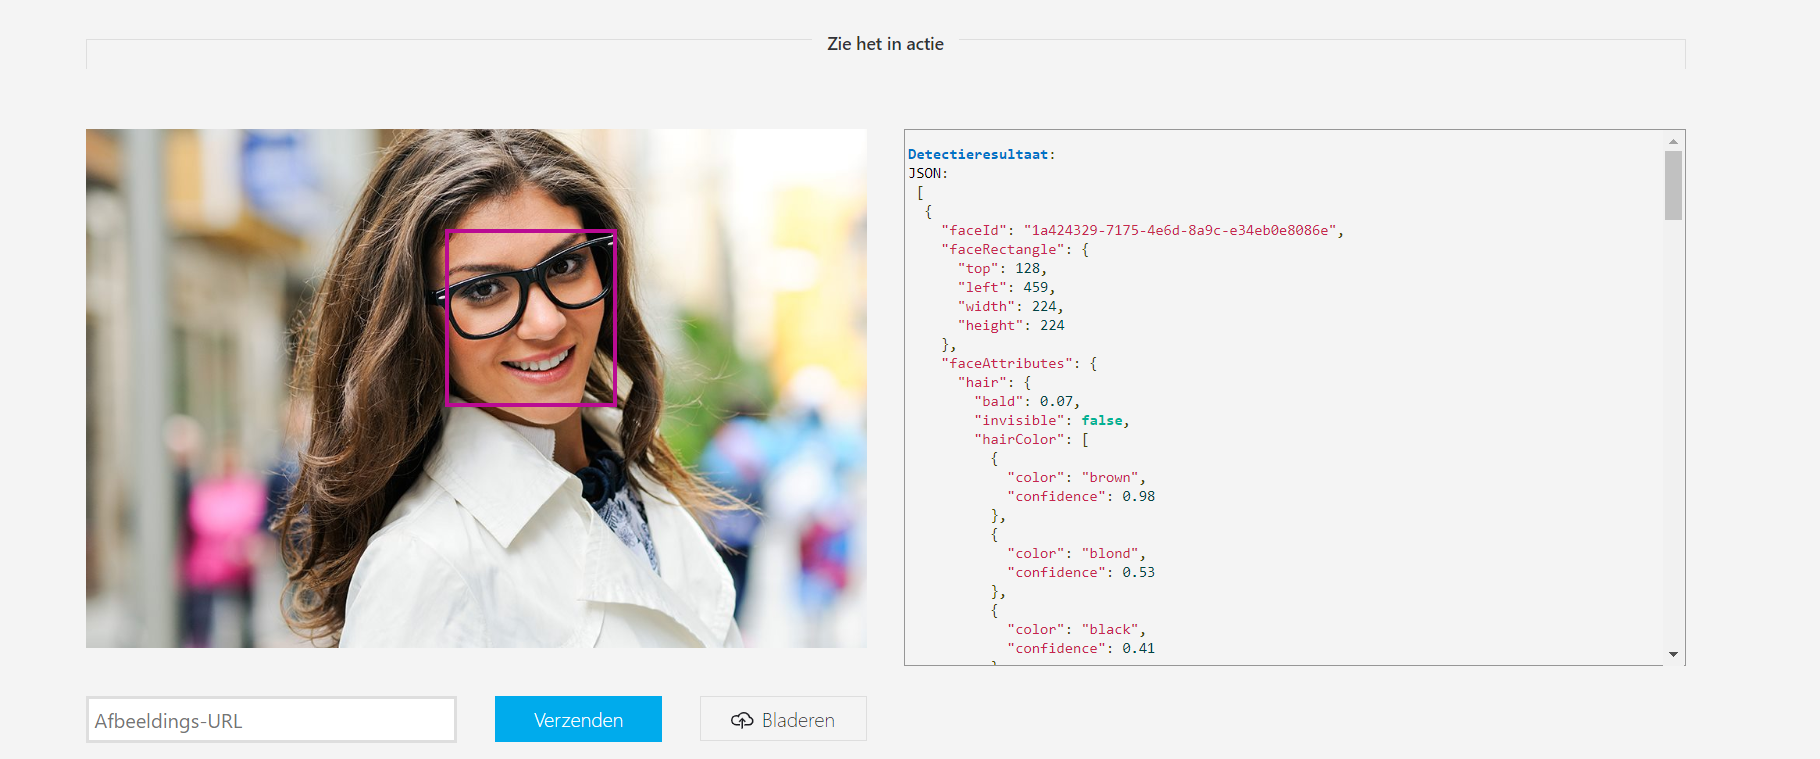
\includegraphics[width=\linewidth]{Face_recogn_micros_1.png}
	\caption{Cognitive services - Face recognition. Links staat een foto met een herkenbaar persoon, rechts een JSON-file als resultaat van Cognitive Services api.}
	\label{fig:cognitive}
\end{figure}

Op \hyperref[fig:cognitive]{figuur 2.5} staat het resultaat van de gezichtsherkenning van Microsoft in werking. Dit is een online demo beschikbaar voor iedereen op de website van Cognitive services. Links op de figuur staat een foto met een duidelijk herkenbaar gezicht. Rechts staat het verwerkte resultaat van een interpretratie van wat in de foto te zien is, automatisch gegenereerd. 

Het eerste herkende element is een face-id. \textbf{Zodra er een face-id aanwezig in het teruggegeven JSON-bestand, betekent dit dat een gezicht herkend is}. Er wordt van uitgegaan dat wanneer er een gezicht op een foto aanwezig is, de foto als persoonlijke data kan aanzien worden. 
Daarnaast zijn nog een heel wat extra elementen (haarkleur, grootte van gezicht, enzoverder) ter beschikking. Deze zijn voorlopig niet van belang, aangezien de bedoeling is om data te kunnen indelen in persoonlijke data/ abstract data, en er daarvoor geen extra elementen zoals haarkleur nodig zijn. 


\subsubsection{Gezichtsherkenning Google cloud}
Met Google Cloud Vision levert Google een zeer gelijkaardige service als de face-api van Microsoft. Opnieuw is een online demo beschikbaar die een voorvertoning geeft van hoe gezichten op foto's herkend worden. We gebruiken dezelfde foto als in \hyperref[fig:cognitive2]{figuur 2.5}. Het resultaat staat in figuur 2.7. De interpretatie is nagenoeg identiek. Het gezicht werd vlot herkend en er is heel wat extra informatie te zien, zoals 'Joy'. 

\begin{figure}[h]
	\includegraphics[width=\linewidth]{FAce_recogn_google2.png}
	\caption{Cognitive services - Face recognition. Links op de figuur de te analyseren foto, rechts een JSON-file met herkende elementen.}
	\label{fig:facerecogn}
\end{figure}


\subsection{Classificatie van foto's en textextractie uit foto's}
Naast tekst beschikken beide google cloud DLP en MS cognitive services ook over herkenning van elementen in foto's, die kunnen geclassificeerd worden. De API herkent bijvoorbeeld een huis. Dit biedt dus de mogelijkheid om ook foto's te gaan filteren op persoonlijke informatie naast gezichten. 


\begin{figure}[h]
	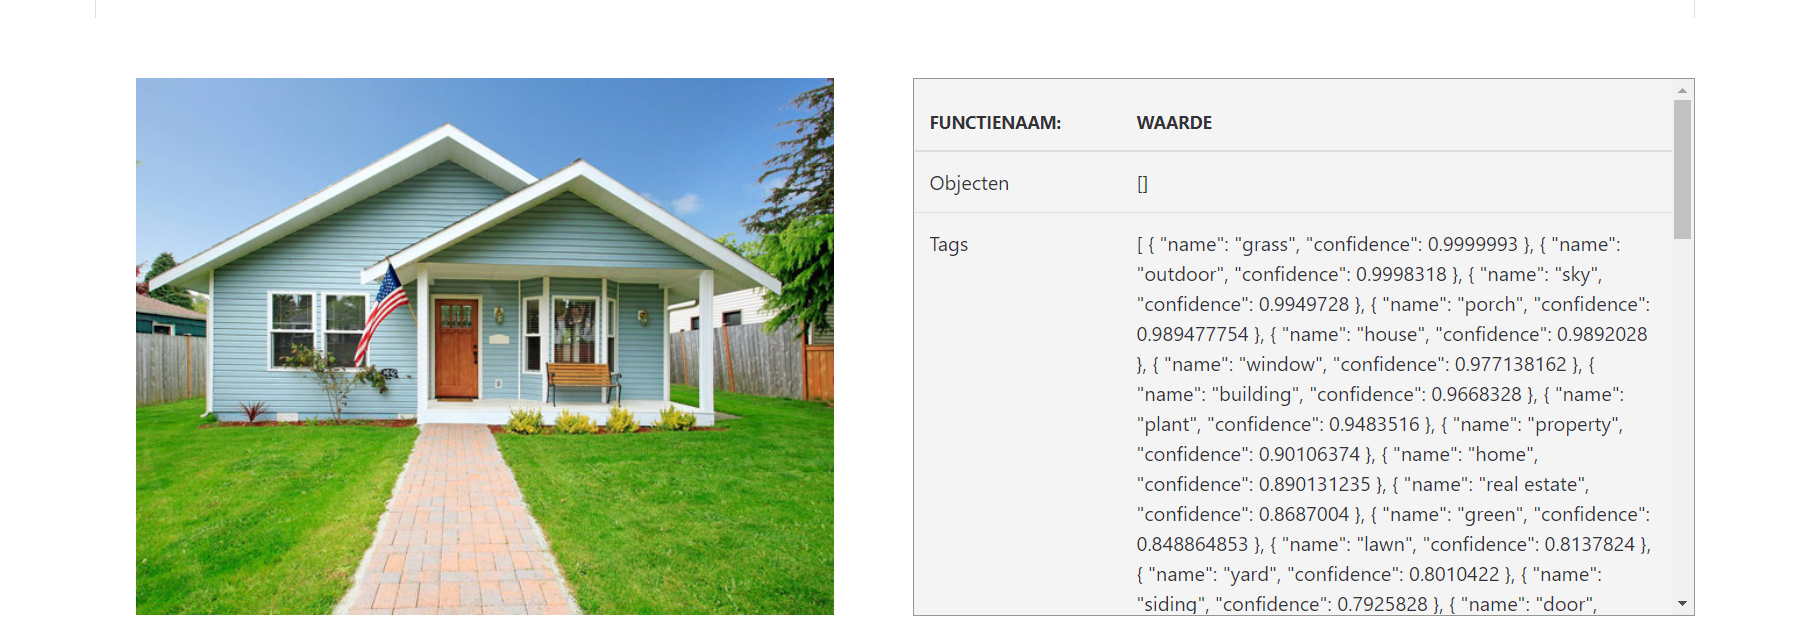
\includegraphics[width=\linewidth]{Image_classification_MS_1.png}
	\caption{Cognitive service - Image classification. Links op de figuur een te analyseren foto, rechts een JSON-file waarin een huis wordt herkend, zekerheid 0.98. }
	\label{fig:Houserecogn}
\end{figure}

\subsection{Automatisch herkennnen persoonlijke informatie uit tekst.}

Naast foto's zal ook tekst geanalyseerd worden. De bedoeling is om uit niet-structurele stukken tekst, personlijke informatie te halen, en er uit te filteren. 
Hiervoor wordt opnieuw gebruik gemaakt van een tool van Microsoft: Language-api met textanalyse. Zie figuur 3.6. 

\begin{figure}[h]
    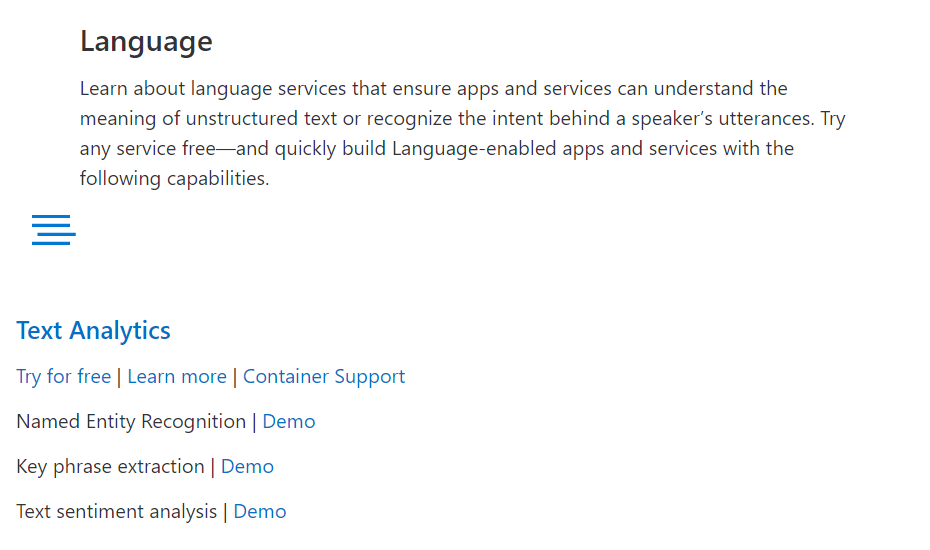
\includegraphics[width=\linewidth]{languageapi.png}
    \caption{Cognitive service - Language API }
    \label{fig:language api}
\end{figure}